\documentclass[11pt,letterpaper]{article}
\usepackage[margin=0.6in]{geometry}
\usepackage{amsmath,amssymb}
\usepackage{tikz}
\usetikzlibrary{arrows.meta,positioning}
\usepackage{xcolor}
\usepackage{fontawesome5}
\usepackage{tcolorbox}
\usepackage{multicol}
\usepackage{enumitem}
\usepackage{hyperref}

\definecolor{primaryblue}{RGB}{41, 98, 255}
\definecolor{accentgreen}{RGB}{0, 150, 136}
\definecolor{warnorange}{RGB}{255, 152, 0}
\definecolor{lightgray}{RGB}{245, 245, 245}

\tcbset{
    conceptbox/.style={colback=primaryblue!5, colframe=primaryblue, boxrule=1pt, arc=3pt, left=5pt, right=5pt, top=5pt, bottom=5pt},
    formulabox/.style={colback=lightgray, colframe=gray!50, boxrule=0.5pt, arc=2pt, left=5pt, right=5pt, top=3pt, bottom=3pt},
    warningbox/.style={colback=warnorange!10, colframe=warnorange, boxrule=1pt, arc=3pt, left=5pt, right=5pt, top=5pt, bottom=5pt},
    appbox/.style={colback=accentgreen!5, colframe=accentgreen, boxrule=1pt, arc=3pt, left=5pt, right=5pt, top=5pt, bottom=5pt}
}

\pagestyle{empty}
\setlength{\parindent}{0pt}
\setlist[itemize]{leftmargin=*, itemsep=1pt, topsep=2pt}

\begin{document}

\begin{center}
{\LARGE\bfseries\color{primaryblue} Chapter 4: Information Theory}\\[3pt]
{\large Entropy, KL Divergence, and Cross-Entropy}
\end{center}
\vspace{-5pt}
\hrule height 2pt
\vspace{8pt}

\begin{multicols}{2}

\begin{tcolorbox}[conceptbox, title={\faLightbulb\ Key Concepts}]
\begin{itemize}
    \item \textbf{Entropy}: Average ``surprise'' of a distribution
    \item \textbf{Cross-Entropy}: Expected surprise using wrong model
    \item \textbf{KL Divergence}: ``Distance'' between distributions
    \item \textbf{Mutual Information}: Shared information between variables
    \item \textbf{Perplexity}: $2^{H(P)}$ --- effective vocabulary size
\end{itemize}
\end{tcolorbox}

\begin{tcolorbox}[formulabox, title={\faCalculator\ Core Formulas}]
\textbf{Entropy:}
\[ H(P) = -\sum_x P(x) \log P(x) \]

\textbf{Cross-Entropy:}
\[ H(P, Q) = -\sum_x P(x) \log Q(x) \]

\textbf{KL Divergence:}
\[ D_{KL}(P \| Q) = \sum_x P(x) \log \frac{P(x)}{Q(x)} \]

\textbf{Key Identity:}
\[ H(P, Q) = H(P) + D_{KL}(P \| Q) \]
\end{tcolorbox}

\columnbreak

\begin{center}
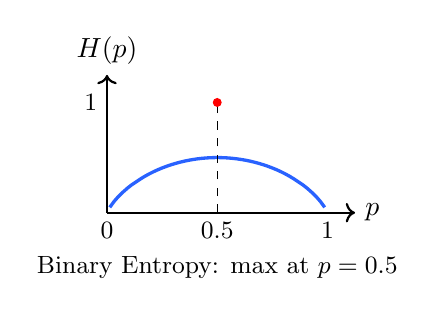
\begin{tikzpicture}[scale=0.7]
    % Binary entropy curve
    \draw[->,thick] (0,0) -- (4.5,0) node[right] {$p$};
    \draw[->,thick] (0,0) -- (0,2.5) node[above] {$H(p)$};

    % Labels
    \node[below] at (0,0) {\small 0};
    \node[below] at (4,0) {\small 1};
    \node[below] at (2,0) {\small 0.5};
    \node[left] at (0,2) {\small 1};

    % Entropy curve
    \draw[primaryblue, very thick, domain=0.05:3.95, samples=50]
        plot (\x, {-(\x/4)*ln(\x/4)/ln(2) - (1-\x/4)*ln(1-\x/4)/ln(2)});

    % Maximum point
    \draw[dashed] (2,0) -- (2,2);
    \filldraw[red] (2,2) circle (2pt);

    \node at (2,-1) {\small Binary Entropy: max at $p=0.5$};
\end{tikzpicture}
\end{center}

\begin{tcolorbox}[appbox, title={\faRobot\ ML Applications}]
\begin{itemize}
    \item \textbf{Cross-Entropy Loss}: Standard classification loss
    \item \textbf{VAE/ELBO}: KL divergence as regularizer
    \item \textbf{Knowledge Distillation}: Match teacher distribution
    \item \textbf{Language Models}: Perplexity measures quality
    \item \textbf{Contrastive Learning}: Maximize mutual information
\end{itemize}
\end{tcolorbox}

\begin{tcolorbox}[warningbox, title={\faExclamationTriangle\ Common Pitfalls}]
\begin{itemize}
    \item KL divergence is \textbf{not symmetric}: $D_{KL}(P\|Q) \neq D_{KL}(Q\|P)$
    \item $D_{KL}$ is undefined if $Q(x)=0$ where $P(x)>0$
    \item Cross-entropy $\neq$ KL divergence (differs by $H(P)$)
    \item Use \textbf{nats} ($\ln$) or \textbf{bits} ($\log_2$) consistently
\end{itemize}
\end{tcolorbox}

\end{multicols}

\vspace{5pt}
\hrule
\vspace{5pt}

\begin{center}
\faGithub\ \textbf{Notebook}: \url{https://github.com/vijaygwu/math-powers-ai/blob/main/notebooks/ch04_information_theory.ipynb}
\end{center}

\end{document}
